% concatenated from ProblemList20260901.tex



%!TEX TS-program = xelatex
\documentclass[11pt]{amsart}
\usepackage{amsmath, amssymb, amsthm}
\usepackage{bm}
\usepackage[numbers]{natbib}
\usepackage{textcomp}
\usepackage{bibentry}
\usepackage{etoolbox}
\usepackage{hyperref}
\hypersetup{
  pdfauthor={Tianyuan Workshop},
  pdftitle={Open Problems in Mathematical Logic},
  pdfsubject={Open Problems},
  colorlinks=true,
  linkcolor=blue,
  citecolor=blue,
  urlcolor=blue
}
\usepackage{lmodern}
\usepackage{tikz}
\usepackage{relsize}
\usepackage{parskip}
\usepackage{enumerate}
\usepackage{textcomp} % For smart quotes
% Prevent vertical stretching
\raggedbottom

% Limit ToC to section level
\setcounter{tocdepth}{1}

% Theorem definitions
\theoremstyle{definition}
\newtheorem{theorem}{Theorem}[section]
\newtheorem{problem}{Problem}[section]
\newtheorem{question}[theorem]{Question}
\newtheorem{proposition}[theorem]{Proposition}
\newtheorem{example}[theorem]{Example}
\newtheorem{remark}[theorem]{Remark}
\newtheorem{definition}[theorem]{Definition}
\newtheorem{fact}[theorem]{Fact}
\newtheorem{notation}[theorem]{Notation}
% Custom definitions
\def\graph{\mathrm{GRAPH}}
\def\itx#1{{\mbox{\textrm{#1}}}}

% Custom commands for abstract formatting
\newcommand{\abstractauthor}[1]{\noindent\textbf{#1}\par\vspace{0.3\baselineskip}}
\newcommand{\abstractbody}[1]{\noindent #1 \par \vspace{\baselineskip}}

% Suppress References in ToC
\makeatletter
\renewcommand{\bibsection}{\vspace{\baselineskip}\noindent\textbf{References}}
\makeatother

%% Store and print affiliations
%\makeatletter
%\def\affiliations{}
%\newcommand{\addaffil}[2]{%
%  \g@addto@macro\affiliations{%
%    \par
%    \ifx\relax#1\relax\else#1\par\fi
%    \ifx\relax#2\relax\else#2\par\fi
%  }}
%\newcommand{\printaffiliations}{%
%  \clearpage
%  \section*{Affiliations}
%  \begin{center}
%    \begin{minipage}{0.95\textwidth}
%      \raggedright
%      \affiliations
%    \end{minipage}
%  \end{center}
%}
%% Suppress default affiliations
%\AtEndDocument{\let\affil@list\@empty}
%\makeatother

%% Patch amsart affiliations output
%\makeatletter
%\patchcmd{\enddocument}
%  {\ifx\@empty\affil@list\else\newpage\begingroup\centering\affil@list\endgroup\fi}
%  {\ifx\@empty\affil@list\else
%     \newpage
%     \begingroup
%     \centering
%     \parskip=0pt
%     \parindent=0pt
%     \small
%     \begin{minipage}{0.1\textwidth}
%       \raggedright
%       \affil@list
%     \end{minipage}
%     \endgroup
%   \fi}
%  {}{}
%\makeatother


\begin{document}

\title[Open Problems in Mathematical Logic]{Open Problems in Mathematical Logic}
\author[2026 Tianyuan Workshop in Definability and Computation]{George Barmpalias}  
\author[]{Su Gao}  
\author[]{Jialiang He}  
\author[]{Takayuki Kihara}  
\author[]{Andre Nies}  
%\author[]{David Schrittesser}  
\author[]{Theodore Slaman}  
\author[]{Chieu-Minh Tran}  
\author[]{Daniel Turetsky}  
\author[]{Philip Welch}  
\author[]{Liang Yu}  
\author[]{Hang Zhang}

%\date{June 2026}



\begin{abstract}
These open problems were presented in the Problem Sessions held during the Tianyuan Workshop on Definability and Computation, June 22-26, 2026. The problems are organized into sections named after their contributors, in the order of their presentations during the workshop. Notes were taken and compiled by Wei Dai, Xiangxi Hu, Yingying Jiang,  Ruiwen Li, Tianhao Wang, Xu Wang, and Jie Zou.
\end{abstract}
\maketitle
\tableofcontents
%\newpage

\section{George Barmpalias}
%\abstractauthor{George Barmpalias}
%\abstractbody{

The following problems concern Turing ideals generated by sufficiently
random reals.

\begin{problem}[Levin, private communications]
        Are the following true?
    \begin{enumerate}
        \item[(1)] Can every chain of random reals in the Turing degrees
        be combined into a single random real?

        \item[(2)] Can every Turing ideal generated by random reals be
        generated by the columns of a single random real?
    \end{enumerate}
\end{problem}

\begin{notation}
If $\alpha\in 2^\omega$, let $\alpha^{(i)}$ denote the real obtained from
$\alpha$ by deleting the digits $\alpha(k)$ at positions $k$ that are
divisible by $2^i$.
\end{notation}

\begin{itemize}
    \item A \emph{chain} is a sequence $(x_i)_{i\in\mathbb{N}}$ of
    reals such that
    \[
        x_i<_T x_{i+1}
    \]
    for every $i\in\mathbb{N}$.

    \item If $B$ is a chain of reals, the Turing ideal generated by
    $B$ is
    \[
        [B]:=\{z:\exists x\in B,\ z\leq_T x\}.
    \]
    In particular, for a chain $(x_i)_{i\in\mathbb{N}}$,
    \[
        [(x_i)]
        :=
        \{z:\exists i,\ z\leq_T x_i\}.
    \]

    \item For each real $\alpha$, define
    \[
        [\alpha]
        :=
        \{z:\exists i,\ z\leq_T\alpha^{(i)}\}.
    \]

    \item The notation $z\approx x$ means that $z$ and $x$ differ
    on finitely many bits.

    \item The real
        $\bigoplus_i x_i$
    is the infinite join of all the reals $x_i$.
\end{itemize}

\medskip
\begin{proposition}[Barmpalias--Zhang, unpublished]
\textit{If $(x_i)_{i\in\mathbb{N}}$ is a sequence of reals and $\bigoplus_{i\leq n} x_i$ is random for each $n$, then there are reals
$z_i\approx x_i$ so that $\bigoplus_i z_i$ is random. The same conclusion holds for $k$-randomness and weak $k$-randomness for each $k\in \mathbb{N}$.}
\end{proposition}

This proposition gives a partial positive answer to Question~1(1) under
the additional assumption of relative randomness. Question~1(2) asks for
the stronger conclusion that the ideal generated by a random chain is
exactly of the form $[\alpha]$ for some random real $\alpha$.

\begin{problem}[Levin]
    Is it true that, for every $X\subseteq 2^\omega$ with $\mu(X)=1$,
    there exists $Y\subseteq 2^\omega$ with $\mu(Y)=1$ such that, for
    every chain $B\subseteq Y$, there is some $\alpha\in X$ satisfying
    $[B]=[\alpha]$?
  \end{problem}

The class $\mathrm{ML}(\emptyset')$
of $\emptyset'$-random reals, equivalently the class of $2$-random reals,
is a special case.

\begin{problem}
    Is there a chain
    $B\subseteq\mathrm{ML}(\emptyset')$
    such that
    $[B]\neq[\alpha]$
    for every $\alpha\in\mathrm{ML}(\emptyset')$?
\end{problem}

There are two obstacles to constructing such a chain. If $\alpha$ is
$2$-random, then the ideal $[\alpha]$ has the following properties:
\begin{enumerate}
    \item[(i)] For every $x\in[\alpha]$, the ideal $[\alpha]$ contains an
    $x'$-random real.

    \item[(ii)] The jumps of the columns $\alpha^{(i)}$ form a chain and,
    in particular, are pairwise distinct.
\end{enumerate}

\begin{problem}
    Toward a negative answer to Levin's Problem 1.2, are the following true?
    \begin{enumerate}
        \item[(1)] Are there $2$-random reals $x<_T z$ such that
        \[
            x'\equiv_T z'?
        \]

        \item[(2)] Are there $2$-random reals $x<_T z$ such that
        \[
            \left|
                K(x\upharpoonright n)-K(z\upharpoonright n)
            \right|
            =
            O(1)?
        \]

        \item[(3)] Is there a Turing ideal $B$ generated by a chain of
        $2$-random reals such that $B$ contains no $x$-random real for
        any $x\in B$?

        \item[(4)] What are the jumps of $2$-random reals?
        See \cite{BDN}. 
    \end{enumerate}
\end{problem}

\begin{problem}
    Is there an injective one-way function on the reals? More precisely,
    is there a partial computable real function $f$ such that
    \begin{enumerate}
        \item[(i)] $f$ is injective and preserves randomness, 

        \item[(ii)] the domain of $f$ has positive Lebesgue measure, and 

        \item[(iii)]
        $f(x)<_T x$
        for a positive-measure set of reals $x$ in the domain of $f$?
    \end{enumerate}
\end{problem}

Such a function can be used to produce a chain of $2$-random reals with
the same jump in the Turing degrees.

\vskip -10pt
\begin{bibentry}{9}
\begin{thebibliography}{9}

\bibitem{BDN} G. Barmpalias, R. Downey, and K. M. Ng, 
\textit{Jump inversions inside effectively closed sets and applications to randomness}, 
The Journal of Symbolic Logic 76 (2011), no. 2, 491--518.

\end{thebibliography}
\end{bibentry}
%}






\bigskip
\bigskip





















\section{Andre Nies}
%\abstractauthor{Andre Nies}
\subsection*{Oligomorphic groups}

Let $M$ be a countably infinite $\omega$-categorical structure in a
finite first-order signature, and let
\[
    G=\operatorname{Aut}(M),
\]
equipped with the topology of pointwise convergence. Let
$\operatorname{Aut}(G)$ denote the group of continuous automorphisms
of the topological group $G$, and let
\[
    \operatorname{Out}(G)
    :=
    \operatorname{Aut}(G)/\operatorname{Inn}(G)
\]
be its outer automorphism group.

\begin{problem}
    Let $M$ be an $\omega$-categorical structure in a first order finite language. Is the group $\operatorname{Out}(G)$  finite?
\end{problem}

For background see \cite{NiesPaolini}, where it is shown that this group is  countable. For some classical examples like $M=(\mathbb{Q},<)$ \cite{Rubin}, the statement of the problem is true; in this case ${\rm Out} (G)$ has two elements, given by the identity and conjugation by $x \mapsto -x$.    

\subsection*{Computability Theory}


Assume throughout that $A,B\subset\mathbb{N}$. One writes 

\[
A \le_{SJT} B
\]

if for every   order function $h$ there exists a uniformly
$B$-c.e. trace $(T_n)$ satisfying that

\[
|T_n|\le h(n)
\]

and

\[
J^A(n)\downarrow
\Longrightarrow
J^A(n)\in T_n.
\]
Also recall that 
\[
A\le_{LR} B
\iff
{\rm MLR}^B\subseteq{\rm MLR}^A.
\]

\begin{problem}
	Does $\le_{SJT}$ imply $\le_{LR}$?
\end{problem}



 We note that  $A\le_{SJT}\emptyset$ implies $A \le_{LR}\emptyset$, namely, every strongly jump traceable set is $K$-trivial, equivalently, low for ML-random.  For background and references, see \cite{GNT}. The authors there give several   characterisations of $\le_{SJT}$ on the $K$-trivials; for instance,  for $A,B$ $K$-trivial,

\[
A\le_{SJT} B
\iff
\forall\,Y\, \omega\text{-c.a. and }Y\in{\rm MLR}
\Bigl(
A\le_T B\oplus Y
\Bigr).
\]


Let Rec denote the class of recursive sets. 


\begin{problem}
    Is there a $\Pi^0_1$ class $C$ such that $|C\cap {\rm Rec}|=\infty$ and $C\cap {\rm Rec}$ is maximally almost disjoint among the recursive sets?
\end{problem}

 
\vskip -12pt

\begin{bibentry}{9}
\begin{thebibliography}{9}

\bibitem{GNT} N. Greenberg, A. Nies and D. Turetsky.  \textit{Characterising SJT reducibility}, The Journal of Symbolic Logic (2026): 1--23.

\bibitem{NiesPaolini}
A.~Nies and G.~Paolini.
\textit{Oligomorphic groups,  their automorphism groups,   and  the  complexity of their isomorphism}, 
\newblock  {Beijing Journal of Pure and Applied Mathematics, in press}.
 Available at {arxiv.org/pdf/2410.02248.pdf}

\bibitem{Rubin} M. Rubin, \textit{On the reconstruction of $\aleph_0$-categorical structures from their automorphism groups},  Proceedings of the London Mathematical Society 3(2) (1994): 225--249.
\end{thebibliography}
\end{bibentry}




\bigskip
\bigskip

\section{Takayuki Kihara}
%\abstractauthor{Takayuki Kihara}
\abstractbody{

The following problems concern a realizability-theoretic refinement of
many-one and Wadge reducibility.

For sets $A,B\subseteq\omega^\omega$, define
\[
    A\leq_m B
\]
if there is a computable function
\[
    \theta\colon\omega^\omega\to\omega^\omega
\]
such that
\[
    x\in A
    \quad\Longleftrightarrow\quad
    \theta(x)\in B
\]
for every $x\in\omega^\omega$. Replacing ``computable'' by
``continuous'' gives Wadge reducibility, denoted by
\[
    A\leq_W B.
\]

For formulas, the truth-preserving map on instances is not sufficient.
The witnesses for the two formulas must also be uniformly convertible.

Let $\alpha\Vdash\varphi(x)$ mean that $\alpha$ is a witness, or
realizer, for the truth of $\varphi(x)$. The witness relation is defined
inductively from the logical structure of $\varphi$; see
\cite[Definition~2.10]{KiharaHierarchy}.

A formula $\varphi$ is realizability-theoretically many-one reducible
to a formula $\psi$, written
\[
    \varphi\leq_m\psi,
\]
if there are computable functions $\eta,r^{-},r^{+}$ such that
\begin{enumerate}
    \item[(1)]
    \[
        \varphi(x)
        \quad\Longleftrightarrow\quad
        \psi(\eta(x));
    \]

    \item[(2)] If $\alpha\Vdash\varphi(x)$, then
    \[
        r^{-}(\alpha,x)\Vdash\psi(\eta(x));
    \]

    \item[(3)] If $\beta\Vdash\psi(\eta(x))$, then
    \[
        r^{+}(\beta,x)\Vdash\varphi(x).
    \]
\end{enumerate}
This is also called \emph{Levin reducibility}; see
\cite[Definition~2.13]{KiharaHierarchy}. Its continuous analogue gives
the corresponding realizability-theoretic version of Wadge
reducibility.

Existentially quantified variables may depend on all preceding
universally quantified variables. For example, a witness for
\[
    \forall a\,\exists b\,\forall c\,\exists d\,
    \forall e\,\exists f\,\forall g\,
    \varphi(a,b,c,d,e,f,g,x)
\]
consists of three functions
\[
    F_0\colon\omega\to\omega,\qquad
    F_1\colon\omega^2\to\omega,\qquad
    F_2\colon\omega^3\to\omega
\]
such that
\[
    \forall a\,\forall c\,\forall e\,\forall g\,
    \varphi\bigl(
        a,F_0(a),
        c,F_1(a,c),
        e,F_2(a,c,e),
        g,x
    \bigr).
\]
Thus, $F_0(a)$ witnesses $b$, $F_1(a,c)$ witnesses $d$, and
$F_2(a,c,e)$ witnesses $f$.

In addition to the ordinary quantifiers $\exists$ and $\forall$, define
\[
    \exists^\infty n\,\varphi(n)
    \quad\Longleftrightarrow\quad
    \forall m\,\exists n\geq m\,\varphi(n),
\]
and
\[
    \forall^\infty n\,\varphi(n)
    \quad\Longleftrightarrow\quad
    \exists m\,\forall n\geq m\,\varphi(n).
\]

A finite sequence
\[
    \overline{Q}
    \in
    \{\exists,\forall,\exists^\infty,\forall^\infty\}^{<\omega}
\]
is called a \emph{quantifier pattern}. If
\[
    \overline{Q}=Q_0Q_1\cdots Q_\ell,
\]
then a formula of the form
\[
    Q_0n_0\,Q_1n_1\cdots Q_\ell n_\ell\,
    \theta(n_0,\ldots,n_\ell,x),
\]
where $\theta$ is bounded, is called an
$\overline{Q}$-formula.

For each quantifier pattern $\overline{Q}$, let
\[
    \langle\overline{Q}\rangle
\]
denote a fixed $\overline{Q}$-complete formula.

Consider
\[
    \mathrm{Bdd}
    :=
    \left\{
        x\in\omega^\omega:
        \exists n\,\forall k\,
        x(k)\leq n
    \right\},
\]
and
\[
    \mathrm{FIN}
    :=
    \left\{
        x\in\omega^\omega:
        \exists n\,\forall m\geq n\,
        x(m)=0
    \right\}.
\]

Although both are classically $\Sigma^0_2$ properties, their witness
structures are different. The first has the quantifier pattern
$\exists\forall$, whereas the second has the pattern
$\forall^\infty$.

The realizability-theoretic classification of
$\Sigma^0_2$ quantifier patterns consists of exactly three degrees:
\[
    \langle\forall^\infty\rangle
    <_m
    \langle\forall^\infty\forall\rangle
    <_m
    \langle\exists\forall\rangle.
\]
The abstract treatment of this classification is given in
\cite{KiharaManyOne}.

The more concrete analysis of the $\Sigma^0_3$ and $\Pi^0_3$ levels is
given in \cite{KiharaHierarchy}. The known numbers of equivalence
classes are as follows:
\begin{enumerate}
    \item[(1)] There is exactly one many-one equivalence class of $\Pi^0_2$ quantifier patterns,
    represented by
    \[
        \forall\exists.
    \]

    \item[(2)] There are exactly three many-one equivalence classes of $\Sigma^0_2$ quantifier
    patterns, represented by
    \[
        \exists\forall,\qquad
        \forall^\infty\forall,\qquad
        \forall^\infty.
    \]

    \item[(3)] There are exactly three many-one equivalence classes of
    $\Sigma^0_3$ quantifier patterns, represented by
    \[
        \exists\forall\exists,\qquad
        \forall^\infty\exists^\infty,\qquad
        \forall^\infty\exists.
    \]

    \item[(4)] There are exactly five many-one equivalence classes of
    $\Pi^0_3$ quantifier patterns, represented by
    \[
        \forall\exists\forall,\qquad
        \exists^\infty\forall^\infty\forall,\qquad
        \exists^\infty\forall,\qquad
        \forall\forall^\infty\forall,\qquad
        \forall\forall^\infty.
    \]
\end{enumerate}

The corresponding classifications at the fourth level are still in
progress.

\begin{problem}
    Determine the equivalence classes of quantifier patterns at the
    fourth level of the arithmetical hierarchy:
    \begin{enumerate}
        \item[(1)] How many $\equiv_m$-equivalence classes of
        $\Sigma^0_4$ quantifier patterns are there?

        \item[(2)] How many $\equiv_m$-equivalence classes of
        $\Pi^0_4$ quantifier patterns are there?

        \item[(3)] How many $\equiv_{dm}$-equivalence classes of
        $\Sigma^0_4$ quantifier patterns are there?
    \end{enumerate}
\end{problem}



\begin{problem}
    Is there a decision procedure which, given quantifier patterns
    \[
        \overline{P},\overline{Q}
        \in
        \{\exists,\forall,\exists^\infty,\forall^\infty\}^{<\omega},
    \]
    decides whether
    \[
        \langle\overline{P}\rangle
        \leq_m
        \langle\overline{Q}\rangle?
    \]
\end{problem}

%Let $x\in\omega^\omega$ code a countable partial order
%\[
%    P_x=(\omega,\leq_{P_x}).
%\]

%Consider the following properties:
%\begin{enumerate}
%    \item[(1)] $\mathrm{IFPO}(x)$ asserts that $P_x$ is ill-founded,
%    that is, there is a function $f\in\omega^\omega$ such that
%    \[
%        f(n+1)<_{P_x}f(n)
%    \]
%    for every $n$.

%    \item[(2)] $\mathrm{Anti}(x)$ asserts that $P_x$ contains an
%    infinite antichain.
%
%    \item[(3)] $\mathrm{NWPO}(x)$ asserts that $P_x$ is not a
%    well-partial-order.

%    \item[(4)] $\mathrm{BadPO}(x)$ asserts that there is a bad sequence
%    in $P_x$:
%    \[
%        \exists f\in\omega^\omega\,
%        \forall i<j\,
 %       \bigl(f(i)\not\leq_{P_x}f(j)\bigr).
 %   \]
%\end{enumerate}

%On the blackboard, the last condition was abbreviated by
%\[
%    \exists f\in\omega^\omega\,
%    \forall n\,
%    \bigl(f(n)\not\leq_{P_x}f(n+1)\bigr).
%\]

%Classically, the failure of the well-partial-order property can be
%described using descending sequences, antichains, or bad sequences.
%From the realizability-theoretic viewpoint, these formulas carry
%different types of witnesses and therefore need not have the same
%many-one degree.

%The blackboard records
%\[
%    \mathrm{IFPO}\equiv_m\mathrm{Anti},
%\]
%and asks for the precise relationship between these problems and
%$\mathrm{BadPO}$.

%For $n\geq 2$, let $\mathrm{IFPO}_n$ and $\mathrm{BadPO}_n$ denote the
%corresponding restrictions to partial orders of width at most $n$.
%For width one, both problems reduce to the ill-founded linear-order
%problem, denoted by $\mathrm{IFLO}$.

%\begin{problem}
%    Determine the realizability-theoretic many-one and Wadge
 %   relationships among the partial-order problems above. In
 %   particular:
%    \begin{enumerate}
%        \item[(1)] Is
%        \[
%            \mathrm{IFPO}\equiv_m\mathrm{BadPO}?
%        \]

%        \item[(2)] For which $m,n\geq 2$ does
%        \[
 %           \mathrm{BadPO}_n
%            \leq_m
 %           \mathrm{IFPO}_m
%        \]
%        hold?

%        \item[(3)] For which $m,n\geq 2$ does
%        \[
%            \mathrm{IFPO}_n
%            \nleq_m
%            \mathrm{BadPO}_m
%        \]
%        hold?
%    \end{enumerate}
%\end{problem}

\vskip -10pt
\begin{bibentry}{9}
\begin{thebibliography}{9}

\bibitem{KiharaManyOne}
T. Kihara,
\textit{Many-one reducibility with realizability}.
arXiv:2403.16027 (2024).

\bibitem{KiharaHierarchy}
T. Kihara,
\textit{The arithmetical hierarchy:
a realizability-theoretic perspective}.
arXiv:2410.15795 (2024).

\end{thebibliography}
\end{bibentry}
}
















\bigskip
\bigskip

\section{Liang Yu}
%\abstractauthor{Liang Yu}
\abstractbody{

A set $A\subseteq\mathbb{R}^2$ is called a \emph{Kakeya set} if, for every
$\alpha\in\mathbb{R}$, there exists $C_\alpha\in\mathbb{R}$ such that
\[
    y=\alpha x+C_\alpha
    \quad\Longrightarrow\quad
    (x,y)\in A
\]
for every $(x,y)\in\mathbb{R}^2$. Equivalently,
\[
    \bigl\{(x,y)\in\mathbb{R}^2:y=\alpha x+C_\alpha\bigr\}
    \subseteq A
\]
for every $\alpha\in\mathbb{R}$.

\begin{problem}
    Is there a Kakeya set $A\subseteq\mathbb{R}^2$ such that
    \[
        x\oplus y\geq_T\emptyset'
    \]
    for every $(x,y)\in A$?
\end{problem}

A Kakeya set $A$ is called \emph{minimal} if every proper subset
$B\subsetneq A$ is not a Kakeya set.

\begin{problem}
    Does every Borel Kakeya set $A$ contain a minimal Kakeya set
    $B\subseteq A$?
\end{problem}

Yinghe Peng has shown that there is a full fine Kakeya set which contains no minimal Kakeya set.
}




\bigskip
\bigskip

\section{Jialiang He}
%\abstractauthor{Jialiang He}
These notes concern two related definability questions in infinite combinatorics and Borel model theory. 

%Throughout, we identify each subset $A\subseteq\omega$ with its characteristic function $\chi_A\in 2^\omega$. Under this coding, $[\omega]^\omega=\{A\subseteq\omega: \text{A is infinite}\}$ is a $G_\delta$, hence Borel, subspace of $2^\omega$. 

%\begin{definition}
%A set $\mathcal A\subseteq[\omega]^\omega$ is called an \emph{independent family} iff for  any pairwise distinct
%\[
%A_1,\ldots,A_n,B_1,\ldots,B_m\in\mathcal A,
%\]
%we have
%\[
%\left|
%A_1\cap\cdots\cap A_n
%\cap
%B_1^c\cap\cdots\cap B_m^c
%\right|=\aleph_0.
%\]
%An independent family $\mathcal A$ is called a \emph{maximal independent family}, if it is maximal with respect to inclusion among independent families.
%\end{definition}

%There is a basic negative theorem is due to Miller.

%\begin{theorem}[Miller {\cite{Miller1989}}]
%There is no $\bm{\Sigma}^1_1$ maximal independent family.
%\end{theorem}

%\begin{definition}
%A family $\mathcal F\subseteq\omega^\omega$ is called an \emph{independent family of functions} if for every $m\geq 1$, for all pairwise distinct
%\[
%f_0,\ldots,f_{m-1}\in\mathcal F,
%\]
%and for all values
%\[
%j_0,\ldots,j_{m-1}\in\omega,
%\]
%the set
%\[
%\left\{
%n\in\omega:
%f_0(n)=j_0,\,
%f_1(n)=j_1,\,
%\ldots,\,
%f_{m-1}(n)=j_{m-1}
%\right\}
%\]
%is infinite.

%An independent family of functions $\mathcal F\subseteq\omega^\omega$ is called \emph{maximal} if there is no $g\in\omega^\omega\setminus\mathcal F$ such that $\mathcal F\cup\{g\}$ is still an independent family of functions.
%\end{definition}

%\begin{theorem}[Miller {\cite{Miller1989}}]
%There is no $\bm{\Sigma}^1_1$ maximal independent family of functions.
%\end{theorem}


\begin{definition}
A set $X\subseteq\mathbb R^2$ is called a \emph{two-point set}, if for every line
$L\subseteq\mathbb R^2$,
\[
|X\cap L|=2.
\]
\end{definition}

\begin{theorem}[Larman {\cite{Larman1968}}]
There is no $F_\sigma$ two-point set.
\end{theorem}

Since every $F_\sigma$ set is Borel, Larman's theorem rules out the lowest
nontrivial possibility in the Borel hierarchy, but it does not settle the following problem.

\begin{problem}
Is there a Borel two-point set?
\end{problem}

Miller showed that, assuming G\"odel's axiom of constructibility $V=L$, there is
a $\bm{\Pi}^1_1$, i.e., coanalytic two-point set \cite{Miller1989}.

\begin{definition}
A \emph{standard Borel space} is a measurable space isomorphic to the Borel space of a Polish space. A \emph{Borel field} is a field $(F, +, \times)$ whose universe is a standard Borel space and whose field operations $+,\times$ are Borel.
\end{definition}

\begin{definition}
Let $F$ be a Borel field. A \emph{Borel algebraically closed extension} of $F$ is a Borel field $K$, together with a Borel injective field homomorphism
\[
\iota:F\hookrightarrow K,
\]
such that $K$ is algebraically closed.
\end{definition}

\begin{problem}[Montalb\'an--Nies {\cite[Question 2.8]{MontalbanNies2013}}]
Does every Borel field have a Borel algebraically closed extension?
\end{problem}

\begin{thebibliography}{99}

\bibitem{Larman1968}
D. G. Larman,
\emph{A problem of incidence},
Journal of the London Mathematical Society
\textbf{43} (1968), 407--409.

\bibitem{Miller1989}
A. W. Miller,
\emph{Infinite combinatorics and definability},
Annals of Pure and Applied Logic
\textbf{41} (1989), no. 2, 179--203.

\bibitem{MontalbanNies2013}
A. Montalb\'an and A. Nies,
\emph{Borel structures: a brief survey},
in \emph{Effective Mathematics of the Uncountable},
Lecture Notes in Logic, vol. 41,
Association for Symbolic Logic, La Jolla, CA, 2013,
124--134.

\end{thebibliography}


\bigskip
\bigskip

\section{Chieu-Minh Tran}
It is about Morley's categoricity in power theorem. 
According to \cite{Mor}, there is the following consequence.
\begin{theorem}
    For a countable theory $T$, if it is $\kappa$ categorial for some $\kappa>\aleph_0$, then it is $\lambda$ categorial for all uncountable $\lambda$.
\end{theorem}
And \cite{CM} replaced $\kappa$ in the above theorem by recursion theoretic complexity (arithmetic degree). Then, the sequel goes to  categoricity without Choice. The first research about this topic date back to \cite{She} shows that we still have the theorem holds if we assume ZF + there is some uncountable well ordered set of reals.
\begin{theorem}{[ZF $+$ there is an uncountable well ordered set
of reals].}

The following conditions on a countable (first order) $T$ are equivalent:
    \begin{enumerate}
        \item $T$ is categorical in some cardinal $\aleph_{\alpha} > \aleph_0$,in $\mathbf V$, of course
        \item $T$ is categorical in every cardinal $\aleph_{\beta} > \aleph_0$,
        in $\mathbf V$, of course
        \item $T$ is, in $\mathbf L[T]$, totally transcendental
        (i.e. $\aleph_0$-stable) with no two cardinal models
        (i.e., for no model $M$ of $T$ and formula
        $\varphi(x,y) \in \mathbf L(\tau_T)$ and
        $\bar a \in {}^{\ell g(\bar y)}M$ do we have
        $\aleph_0 \leq |\varphi(M,\bar a)| < \|M\|$
        and $\|M\|$ is a cardinal, i.e. the set of elements of $M$ is well-orderable hence its power is a cardinal)
        \item If $\mathbf V' \subseteq \mathbf V$ is a transitive class extending
        $\mathbf L$, $T \in \mathbf V'$ and $\mathbf V'$ satisfies ZFC, then the conditions in (3) hold
        \item For some $\mathbf V'$ clause (4) holds.
    \end{enumerate}
\end{theorem}

However, for non-well-ordered cardinals, the situation deteriorates quickly. The sequel is the following.
For such a theory $T$, we want to show it is very close to a stongly minimal $T'$. It is like a vector space over fixed field or algebraically closed field. And since there is no well order, it is hard to take a basis and match them to one another. So there is the question.
\begin{problem}
    For vector space over fixed $\mathbb{K}$, is choose a basis require the full Axiom of Choice?
\end{problem}

\vskip -12pt
\begin{bibentry}{}
\begin{thebibliography}{9}
\bibitem{Mor} M. Morley, \textit{Categoricity in power}, Transactions of the American Mathematical Society 114 (1965), 514-538.
\bibitem{CM} J.L Goh, C.-M. Tran, \textit{Categoricity without power}, 2026, arXiv:2605.00697
\bibitem{She} S. Shelah, \textit{Model theory without choice: Categoricity}, The Journal of Symbolic Logic 74 (2) (2009): 361-401.

\end{thebibliography}
\end{bibentry}







\bigskip
\bigskip


\section{Theodore Slaman}
   In 1954, \cite{Mar} shows that for $E\subseteq \mathbb{R}^2$ an analytic set with Hausdorff dimension 1. Then, for almost all $\theta$, the projection of $E$ onto a line with slope $\theta$ has Hausdorff dimension 1. Later in 1969, \cite{Dav} shows that CH could imply there is some $E\subseteq \mathbb{R}^2$ with Hausdorff dimension 1 and for all $\theta$, projection of $E$ onto a line of slope $\theta$ has Hausdorff dimension 0. \par
   \begin{problem}
       Is there a Davies example provably in ZFC?
   \end{problem}
  
  \vskip -10pt
\begin{bibentry}{9}
\begin{thebibliography}{9}
\bibitem{Mar} J. M. Marstrand, \textit{The dimension of Cartesian product sets}, Mathematical Proceedings of the Cambridge Philosophical Society  50 (1954), no. 2, 198-202. 
\bibitem{Dav} R. O. Davies, \textit{Measures of Hausdorff type}, Journal of the London Mathematical Society s2-1 (1969), no. 1, 30-34.
\end{thebibliography}
\end{bibentry}


































\bigskip
\bigskip


\section{Hang Zhang}
The following questions are motivated by the problem whether hyper-\linebreak hyperfiniteness implies hyperfiniteness. 

Let $M$ be a   countable model for a sufficiently large
 fragment of ZFC. Suppose that a partial order $P$ is in $M$. Define the space $Gen^P_M$ of $M$-generics for $P$ by 
 
$$Gen^P_M= \{G \subseteq P:  \mbox{ $G$ is an $P$-generic filter over $M$}\}.$$

If we   identify $Gen^P_M$
 as a subspace of $2^P$  with the product topology, then $Gen^P_M$ is $G_\delta$ in  $2^P$ and thus a Polish space. See \cite{smythe} for details. Define $G\sim H $ if and only if $M[G]=M[H]$. Consider the equivalence relation $\sim$ on $Gen^P_M$.
 
\begin{example}
    (Calderoni--Sinapova \cite{CS}) Let $M$ be a countable model for large fragment ZFC.
Suppose $M\models \kappa$ is measurable (witnessed by $\mathcal{U}$). If $M\models \mathbb{P}=\{(s,A): s=\langle s_0,\dots, s_n\rangle,\ n\in\omega,\ A\in\mathcal{U}\}$, with order
$(s,A)\leq (t,B) \iff t\subseteq s \land s\setminus t\subseteq B \land A\subseteq B$.
Then for any generic sequences $\vec{\alpha}, \vec{\beta}$ of $\mathbb{P}$ over $M$, 
\[
M[\vec{\alpha}]=M[\vec{\beta}]\iff \exists N\ \forall n>N\ \ \alpha(n)=\beta(n) \tag{$*$}.
\]
\end{example}

\begin{problem}
    Find more models $M$ and forcing notions $\mathbb{P}\in M$ such that $(*)$ is true.
\end{problem}
\begin{remark}[{\cite[Theorem 3.1]{smythe}}]
If $\mathbb{P}=\mathbb{C}$ (Cohen forcing), then "$x\thicksim y\iff M[x]=M[y]$" is hyper-hyperfinite.
\end{remark}
\begin{problem}[{\cite[Question 5.2]{smythe}}]
 Is $\thicksim$ hyperfinite? 
\end{problem}
\begin{problem}
    Suppose there are a model $M$ and a forcing notion $\mathbb{P}\in M$ such that $(*)$ is true. Can we deduce that $M\models [\exists\  \text{a large cardinal}]$?
\end{problem}
\begin{remark}
    If $$\langle0,\cdots,0,1,0,\cdots,0,1,1,0\cdots\rangle$$
is Cohen, then $$\langle1,\cdots,1,0,1,\cdots,1,0,0,1\cdots\rangle$$ is also Cohen. Notice that these two Cohen reals lead to the same  forcing extension. So Cohen forcing does not satisfy (*) for any $M$.
\end{remark}    

\vskip -10pt
\begin{bibentry}{9}
\begin{thebibliography}{9}
\bibitem{smythe}I. B. Smythe, \textit{Equivalence of generics}, Archive for Mathematical Logic 61(2022), 795--812.
\bibitem{CS} F. Calderoni, D. Sinapova, \textit{Forcing, genericity and countable Borel equivalence relations}, preprint, 2025, arXiv: 2503.14811.
\end{thebibliography}
\end{bibentry}































\bigskip
\bigskip



\section{Daniel Turetsky}
\quad If $\mathbf{a}<\mathbf{b}<\mathbf{c}$ are Turing degrees, and $\mathbf{a}$, $\mathbf{c}$ contain different Martin-L\"of randoms, then must $\mathbf{b}$ contain one? The answer is no.
\begin{problem}
    Does this hold with a larger degree notion, for example, LR-degrees?
\end{problem}























\bigskip
\bigskip





\section{Philip Welch}
    \quad First we recall some basic notions in \cite{Welch}. Let $\beta$ be an ordinal. Suppose $M$ is a nonstandard model of $\mathsf{KP}$, and $\{\zeta_i:i\in\mathbb{N}\}$, $\{s_i:i\in\mathbb{N}\}$ are sequences of $M$-ordinals. If $\left(M,\{\zeta_i:i\in\mathbb{N}\},\{s_i:i\in\mathbb{N}\}\right)$ satisfies the following:
    \begin{enumerate}
        \item $M$ extends $L_\beta$;
        \item for all $i$, $\zeta_i<\zeta_{i+1}<\beta$ and $s_{i+1}<^Ms_i$;
        \item for all $i$, $L_{\zeta_i}\prec_{\Sigma_{m+1}} L_{s_i}^M$;
        \item for all $i$, $L_{s_{i+1}}^M\prec_{\Sigma_{m-1}} L_{s_i}^M$,
    \end{enumerate}
    then we call this triple a strong $\Sigma_{m+1}$-nesting on $\beta$. And we say $\beta$ supports a strong $\Sigma_{m+1}$-nesting if there exist such nonstandard model $M$ of $\mathsf{KP}$ and sequences $\{\zeta_i:i\in\mathbb{N}\},\{s_i:i\in\mathbb{N}\}$ of $M$-ordinals for $L_\beta$.

    \quad We call a function $\Phi:\mathbb{R}\to\mathbb{R}$ an operator ($\mathcal{P}(\mathbb{N})$ and $\mathbb{R}$ are identified). An operator $\Phi$ is said to be 
    \begin{enumerate}
        \item $\bm{\Pi}_m^1$ if there exists a $\bm{\Pi}_m^1$ formula $\phi$ and a parameter $Y$ such that
        $$\forall n\,\forall X\left(n\in\Phi(X)\leftrightarrow\phi(n,X,Y)\right);$$
        \item monotone if $X\subseteq Y$ implies $\Phi(X)\subseteq\Phi(Y)$.
    \end{enumerate}
    The axiom $\bm{\Pi}_{m+1}^1\mathsf{-MI}$ asserts that for every monotone $\bm{\Pi}_{m+1}^1$ operator $\Phi$, there is some prewellordering $W$ such that for all $a\in\textrm{field}(W)=\textrm{dom}(W)\cup\textrm{ran}(W)$, we have 
    $$W_a=\Phi(W_{<a}).$$
    Here
    \begin{align*}
        &W_a=\{b:a<_Wb\},\\
        &W_{<a}=\bigcup\{W_b:b<_Wa\}.
    \end{align*}
    Note that an operator $\Phi$ can be iterated by setting $\Phi^0=\emptyset, \Phi^{<\alpha}=\bigcup_{\gamma<\alpha}\Phi^\gamma$ and $\Phi^\alpha=\Phi(\Phi^{<\alpha})$. Put $\Phi^\infty=\bigcup_\alpha\Phi^\alpha$. We can see that the field of $W$ is $\Phi^\infty$.
\begin{problem}
    If $L_\beta\models\mbox{$\mathit{V}=\mathit{HC}$}$, then
    \begin{align*}
       \left(\mathcal{P}(\omega)\cap L_\beta\models\bm{\Pi}_{m+1}^1\mathsf{-MI}\,\right)\iff\beta\mbox{ supports a strong }\Sigma_{m+1}\textrm{-nesting}.
    \end{align*}
\end{problem}


\vskip -10pt
\begin{bibentry}{9}
\begin{thebibliography}{9}
\bibitem{Welch} J. P. Aguilera, P. D. Welch, \textit{Determinacy on the edge of second-order arithmetic, I}, Journal of the London Mathematical Society 113(3) (2026), e70456.
\end{thebibliography}
\end{bibentry}






























\bigskip
\bigskip































\bigskip
\bigskip




\section{Su Gao}
%\abstractauthor{Su Gao}
\quad This question is about equivalence relations given by complete first-order theories. The question has been circulating in the community since early 2000s.

Consider a complete first order theory $T$ in a countable language. Let
$\mathrm{Mod}(T)$ be the Polish space of countable models of $T$ with universe $\omega$. Let $\cong\restriction_{\mathrm{Mod}(T)}$ denote the isomorphism relation on $\mathrm{Mod}(T)$. Recall two basic equivalence relations in descriptive set theory:
\begin{enumerate}
    \item $=$ is the identity relation on $\mathbb{R}$;
    \item $=^+$ is the equivalence relation on $\mathbb{R}^\omega$ that $(x_n)_{n\in\omega}=^+(y_n)_{n\in\omega}$ if they represent the same countable subset of reals, i.e., if
    $$ \{x_n\colon n\in\omega\}=\{y_n\colon n\in\omega\}.$$ 
\end{enumerate}

Also note the following fact:
\begin{fact}
    (1) There is a complete theory $T$ such that $=$ is Borel bi-reducible to $\cong\restriction_{\mathrm{Mod}(T)}$. For example, $T$ can be chosen as the theory of the equivalence relation on $\omega$ with infinitely many equivalence classes of any finite size.\\
   (2) There is a complete theory $T'$ such that $=^+$ is Borel bi-reducible to $\cong\restriction_{\mathrm{Mod}(T')}$. For example, $T'$ can be chosen as the theory of infinitely many independent equivalence relations on $\omega$ and every equivalence relation has infinitely many equivalence classes of any finite size.
\end{fact}
So we have the following natural question:
\begin{problem}\label{prob:12.2}
    Does there exist a complete first-order theory $T$ in a countable language such that $=\ <_B\ \cong\restriction_{\mathrm{Mod}(T)}\ <_B\ =^+$?
\end{problem}

\begin{remark}
    Note that $=\ <_B\ =^+$, and there are equivalence relations strictly between them. For example, $E_0,E_\infty,E^\omega_0$. So, they are natural candidates for the complexity of $\cong\restriction_{\mathrm{Mod}(T)}$ for some $T$ if the problem has a positive answer.
\end{remark}

There have been some research (e.g. \cite{Mar07, Koe09, CK10, RS17}) on this problem and more generally on the isomorphism relation $\cong\restriction_{\mathrm{Mod}(T)}$ in the Borel reducibility sense. In particular, Dave Marker showed in \cite{Mar07} that if $S(T)$ (the Stone space of $T$-types) is uncountable, then $T$ is not an example for Problem~\ref{prob:12.2}.


\vskip -12pt 
\begin{bibentry}{9}
\begin{thebibliography}{9}
\bibitem{Mar07} D. Marker, \textit{The Borel complexity of isomorphism for theories with many types}, Notre Dame Journal of Formal Logic 48 (2007), no. 1, 93--97.
\bibitem{Koe09} M. Koerwien, \textit{Comparing Borel reducibility and depth of an $\omega$-stable theory}, Notre Dame Journal of Formal Logic 50 (2009), no. 4, 365--380.
\bibitem{CK10} S. Coskey, R. Kossak, \textit{The complexity of classification problems for models of arithmetic}, Bulletin of Symbolic Logic 16 (2010), no. 3, 345--358.
\bibitem{RS17} R. Rast, D. Singh Sahota, \textit{The Borel complexity of isomorphism for o-minimal theories}, The Journal of Symbolic Logic 82 (2017), no. 2, 453--473.
\end{thebibliography}
\end{bibentry}




\end{document}










\section{David Schrittesser}
\quad Let us first recall two classes of groups. They are both subgroups of $S_\infty$ and share similar flavor. 

\begin{definition}
    We say a subgroup $G\leq S_\infty$ is \emph{cofinitary} if 
    $$\forall g\in G\setminus \{1\},\ \text{fix}(g)=\{n\in\omega|\ g(n)=n\}$$
    is finite.
   
    We say a group $G\leq S_\infty$ is \emph{maximal cofinitary} if for every proper extension $G\lneq G'\leq S_\infty$, $G'$ is not cofinitary. 
\end{definition}
\begin{definition}
    We say a subgroup $G\leq S_\infty$ is \emph{finitely periodic} if 
    $\forall g\in G\setminus \{1\}$, $\langle g\rangle_{S_\infty}$ only has finitely many finite orbits.
    
    Similarly, we say a group $G\leq S_\infty$ is \emph{maximal finitely periodic} if for every proper extension $G\lneq G'\leq S_\infty$, $G'$ is not finitely periodic. 
\end{definition}

Maximal cofinitary groups have been studied by Bart Kastermans in \cite{Kas}. It is known that maximal cofinitary groups cannot be $K_\sigma$, abelian, and there is a coanalytic maximal cofinitary group if assuming the axiom of constructibility. So we can ask similar questions for maximal finitely periodic groups:
\begin{problem}
    Is there a countable or $K_\sigma$ or just Borel maximal finitely periodic group?
\end{problem}
\vskip -12pt 
\begin{bibentry}{9}
\begin{thebibliography}{9}
\bibitem{Kas} B. Kastermans, \textit{The complexity of maximal cofinitary groups}, Proceedings of the American Mathematical Society 137(1) (2009), 307–316.
\end{thebibliography}
\end{bibentry}



































%!TEX TS-program = xelatex
\documentclass[11pt]{amsart}
\usepackage{amsmath, amssymb, amsthm}
\usepackage[numbers]{natbib}
\usepackage{textcomp}
\usepackage{bibentry}
\usepackage{etoolbox}
\usepackage{hyperref}
\hypersetup{
  pdfauthor={Tianyuan Workshop},
  pdftitle={Open Problems in Computability Theory and Descriptive Set Theory},
  pdfsubject={Open Problems},
  colorlinks=true,
  linkcolor=blue,
  citecolor=blue,
  urlcolor=blue
}
\usepackage{lmodern}
\usepackage{tikz}
\usepackage{relsize}
\usepackage{parskip}
\usepackage{enumerate}
\usepackage{textcomp} % For smart quotes
% Prevent vertical stretching
\raggedbottom

% Limit ToC to section level
\setcounter{tocdepth}{1}

% Theorem definitions
\theoremstyle{definition}
\newtheorem{theorem}{Theorem}
\newtheorem{problem}[theorem]{Problem}
\newtheorem{proposition}[theorem]{Proposition}

% Custom definitions
\def\graph{\mathrm{GRAPH}}
\def\itx#1{{\mbox{\textrm{#1}}}}

% Custom commands for abstract formatting
\newcommand{\abstractauthor}[1]{\noindent\textbf{#1}\par\vspace{0.3\baselineskip}}
\newcommand{\abstractbody}[1]{\noindent #1 \par \vspace{\baselineskip}}

% Suppress References in ToC
\makeatletter
\renewcommand{\bibsection}{\vspace{\baselineskip}\noindent\textbf{References}}
\makeatother

%% Store and print affiliations
%\makeatletter
%\def\affiliations{}
%\newcommand{\addaffil}[2]{%
%  \g@addto@macro\affiliations{%
%    \par
%    \ifx\relax#1\relax\else#1\par\fi
%    \ifx\relax#2\relax\else#2\par\fi
%  }}
%\newcommand{\printaffiliations}{%
%  \clearpage
%  \section*{Affiliations}
%  \begin{center}
%    \begin{minipage}{0.95\textwidth}
%      \raggedright
%      \affiliations
%    \end{minipage}
%  \end{center}
%}
%% Suppress default affiliations
%\AtEndDocument{\let\affil@list\@empty}
%\makeatother

%% Patch amsart affiliations output
%\makeatletter
%\patchcmd{\enddocument}
%  {\ifx\@empty\affil@list\else\newpage\begingroup\centering\affil@list\endgroup\fi}
%  {\ifx\@empty\affil@list\else
%     \newpage
%     \begingroup
%     \centering
%     \parskip=0pt
%     \parindent=0pt
%     \small
%     \begin{minipage}{0.1\textwidth}
%       \raggedright
%       \affil@list
%     \end{minipage}
%     \endgroup
%   \fi}
%  {}{}
%\makeatother


\begin{document}

\title[Open Problems in Computability Theory and DST]{Open Problems in Computability Theory and Descriptive Set Theory}
\author[G. Barmpalias]{George Barmpalias}
%\address{State Key Lab of Computer Science, Institute of Software Chinese Academy of Sciences, Beijing, China}
%\email{barmpalias@gmail.com}
\author[N. Bazhenov]{Nikolay Bazhenov}
%\address{Sobolev Institute of Mathematics, pr. Akad. Koptyuga 4, Novosibirsk, 630090 Russia}
%\email{bazhenov@mail.math.nsc.ru}
\author[C. T. Chong]{Chi Tat Chong}
%\address{Department of Mathematics, National University of Singapore, Singapore, 119076, Singapore}
%\email{chongct@nus.edu.sg}
\author[W. Dai]{Wei Dai}
%\address{School of Mathematical Sciences and LPMC, Nankai University, Tianjin 300071, P.R. China}
%\email{weidai@nankai.edu.cn}
\author[S. Gao et al.]{Su Gao}
%\address{School of Mathematical Sciences and LPMC, Nankai University, Tianjin 300071, P.R. China}
%\email{sgao@nankai.edu.cn}
\author[]{Jun Le Goh}
%\address{Department of Mathematics, National University of Singapore, Singapore 119076, Singapore}
%\email{gohjunle@nus.edu.sg}
\author[]{Jialiang He}
%\address{School of Mathematics, Sichuan University, Chengdu 610064, China}
%\email{jialianghe@scu.edu.cn}
\author[]{Keng Meng Selwyn Ng}
%\address{Division of Mathematical Sciences, School of Physical and Mathematical Sciences, Nanyang Technological University, 21 Nanyang Link, Singapore, 637371, Republic of Singapore}
%\email{kmng@ntu.edu.sg}
\author[]{Andre Nies}
%\address{Department of Computer Science, University of Auckland, Private Bag 92019, Auckland, New Zealand}
%\email{andre@cs.auckland.ac.nz}
\author[]{Theodore Slaman}
%\address{Department of Mathematics, University of California, Berkeley}
%\email{slaman@math.berkeley.edu}
\author[]{Riley Thornton}
%\address{CMU Math Department, 5000 Forbes Ave, Pittsburgh PA, 15232}
%\email{rthornto@andrew.cmu.edu}
\author[]{Wei Wang}
%\address{Institute of Logic and Cognition and Department of Philosophy, Sun Yat-Sen University, Guangzhou, China}
%\email{wwang.cn@gmail.com}
\author[]{Jing Yu}
%\address{Shanghai Center for Mathematical Sciences, Fudan University, Shanghai, China}
%\email{jyu@fudan.edu.cn}
\author[]{Liang Yu}
%\address{Department of Mathematics, Nanjing University, Jiangsu Province 210093, P. R. of China }
%\email{yuliang.nju@gmail.com}


\date{June 2025}



\begin{abstract}
These open problems were presented in the Problem Sessions held during the Tianyuan Workshop on Computability Theory and Descriptive Set Theory, June 16-20, 2025. The problems are organized into sections named after their contributors, in the order of their presentations during the workshop. Notes were taken and compiled by Wei Dai, Feng Li, Ruiwen Li, Ming Xiao, Xu Wang, Víctor Hugo Yañez Salazar, and Yang Zheng.
\end{abstract}
\maketitle
\tableofcontents
%\newpage

\section{Theodore Slaman}
%\abstractauthor{Theodore Slaman}
\abstractbody{
Given $A\subseteq \mathbb{R}$. Define
$$I(A)=\{f \text{ gauge function } : H^f(A)>0\}.$$

\begin{problem}
    Natural questions about $A \mapsto I(A)$:
    \begin{enumerate}
        \item Does the range of $I$ have the same cardinality as $2^{\mathbb{R}}$? (Seems yes under GCH.)
        \item If we consider the closed set $C$, $I(C)$ is arithmetic ($\mathbf{\Sigma}_2^0$). What's the complexity of the set
$$\big\{\mathbf{\Sigma}_2^0 \text{ formula } \varphi : \varphi \text{ defines an } I(C) \text{ for some } C\big\}?$$ Is it $\mathbf{\Sigma}_2^1$-complete? (It is $\mathbf{\Pi}_1^1$-hard.)
        \item Is the answer to "Borel hierarchy is proper w.r.t. the range of $I$" independent of ZFC?
        \item Is it consistent with ZFC that for every $f$ and $A\subseteq \mathbb{R}$, if $H^f(A)>0$, then there is a subset $A_0$ such that $H^f(A_0)$ is finite and positive?
    \end{enumerate}
\end{problem}
}
\begin{bibentry}{9}
\begin{thebibliography}{9}
\bibitem{RF} C. A. Rogers and K. Falconer, Hausdorff Measures, 2nd ed. Cambridge Mathematical Library. Cambridge University Press, Cambridge, 1998.
\bibitem{F} K. Falconer, Fractal Geometry: Mathematical Foundations and Applications. John Wiley \& Sons, Ltd, 2003.
\bibitem{} L. Crone, L. Fishman, and S. Jackson, \textit{Equivalence relations and determinacy}. Journal of Mathematical Logic 22 (2022), Article 2250003.
\end{thebibliography}
\end{bibentry}

\section{George Barmpalias}
%\abstractauthor{George Barmpalias}
\abstractbody{
\begin{problem}
    Let $L_x=\{z : z \leq_K^+ x\}$ and $U_x=\{z : z \geq_K x\}$. Are the following true?
    \begin{enumerate}
        \item[(1)] $L_x$ is countable iff $\liminf_{n\to\infty}(K(x\upharpoonright n)-K(n))<\infty$;
        \item[(2)] $U_x$ is countable iff $\liminf_{n\to\infty}(K(n)+n-K(x\upharpoonright n))<\infty$.
    \end{enumerate}
\end{problem}

\begin{problem}
    Are the following true?
    \begin{enumerate}
        \item[(1)] For any c.e. set $A$, there exists a c.e. set $D\subseteq 2\mathbb{N}$, such that $A\equiv_{rK}D$ and $C(A\upharpoonright n|D\upharpoonright n)=C(D\upharpoonright n|A\upharpoonright n)=O(1)$;
        \item[(2)] For all $x$, there is a random $z$ such that $z \geq_{rK} x$ (or $z \geq_K x$).
    \end{enumerate}
\end{problem}

Consider the Even Number Game defined in \cite{Ba}. Given a natural number $k\geq 2$, the game $G_k$ is a game with two players who take turns to play natural numbers. Player 1 plays a set $A$ of $k$ integers where none of the members of $A$ has been played by her before; then Player 2 plays an even number between $\min(A)$ and $\max(A)$ (inclusive) which has not been played by him before. Player II loses when he has no legal moves.

It was shown in \cite{Ba} that for $k=2,3$, Player 1 has a winning strategy in the game $G_k$. For $k\geq 4$, this is unknown.

\begin{problem}
    For $k\geq 4$, does Player 1 have a winning strategy in the game $G_k$?
\end{problem}

\begin{bibentry}{9}
\begin{thebibliography}{9}
\bibitem{Ba} G. Barmpalias, X. Zhang, and B. Zhan, \textit{Compression of enumerations and gain}. arXiv:2304.03030 (2023).
\end{thebibliography}
\end{bibentry}

}

\section{Jun Le Goh}
%\abstractauthor{Jun Le Goh}
\abstractbody{
Recall that \textbf{WF} is the collection of all well-founded trees on $\omega$ and \textbf{UB} is the collection of all trees on $\omega$ which have a unique infinite branch.
It is known that \textbf{WF} and \textbf{UB} are both coanalytic complete.

Saint Raymond \cite{Raymond} proved in 2007 that (\textbf{WF}, \textbf{UB}) is a coanalytic complete pair using pure Descriptive Set Theory methods, i.e., for every disjoint pair $(A,B)$ of coanalytic sets in the Baire space $\omega^\omega$, there is a continuous function $f : \omega^\omega \to \omega^\omega$ such that $A = f^{-1}[\text{\textbf{WF}}]$ and $B = f^{-1}[\text{\textbf{UB}}]$.

Using recursion theory, Goh proved that any coanalytic separator of \textbf{WF} and \textbf{UB} is coanalytic complete. The method also proves Saint Raymond's theorem.
\begin{problem}
    Can this be proved using Descriptive Set Theoretic methods?
\end{problem}

\begin{bibentry}{9}
\begin{thebibliography}{9}
\bibitem{Raymond} J. Saint Raymond, \textit{Complete pairs of coanalytic sets}. Fundamenta Mathematicae 194 (2007), 267--281.
\end{thebibliography}
\end{bibentry}
}


\section{Liang Yu}{}
%\abstractauthor{Liang Yu}
\abstractbody{
\begin{problem}[Downey--Hirschfeldt--Miller--Nies \cite{DHMN}]
    Is there an $x$ such that $\Omega^x \geq_T 0^{''}$ where
    $$\Omega^x = \sum_{\sigma \in 2^{<\omega}} 2^{-K^x(\sigma)}$$
    and
    $$K^x(\sigma) = \min\{|\tau| : U^x(\tau) = \sigma\}?$$
\end{problem}

Related to this question, Yu and Zhao proved the following proposition:

\begin{proposition}[Yu--Zhao]
    $\forall y \exists x \, \Omega^x \oplus 0^{'} \geq_T y$.
\end{proposition}

\begin{theorem}[Velickovic--Woodin \cite{VM}]
    If $A$ is $\mathbf{\Sigma}_1^1$ and $\sup\{\omega_1^{CK(x)} : x \in A\} = \omega_1$, then $\forall \gamma \exists x_0, x_1, x_2, x_3 \in A$,
    $$\gamma \leq_h x_0 \oplus x_1 \oplus x_2 \oplus x_3.$$
\end{theorem}
\begin{problem}
    \begin{enumerate}[(a)]
        \item Is there a recursion theoretical proof for the above theorem of Velickovic--Woodin?
        \item Is the following true: For any $\Sigma_1^1(y)$ set $A$, if there is $x \in A$ such that $\omega_1^{CK(x)} > \omega_1^{CK(y)}$, then the Velickovic--Woodin theorem holds for $A$?
    \end{enumerate}
\end{problem}

\begin{bibentry}{9}
\begin{thebibliography}{9}
\bibitem{DHMN}
R. Downey, D. R. Hirschfeldt, J. S. Miller, A. Nies,
\textit{Relativizing Chaitin's halting probability}. Journal of Mathematical Logic 5 (2005), no. 2, 167--192.

\bibitem{VM} B. Velickovic and W. H. Woodin, \textit{Complexity of reals in inner models of set theory}. Annals of Pure and Applied Logic 92 (1998), 283--295.
\end{thebibliography}
\end{bibentry}

}


\section{Wei Wang}
%\abstractauthor{Wei Wang}
\abstractbody{
We start with some definitions.

A tree $T \subseteq 2^{<\omega}$ is \emph{positive} if $[T]$ has measure $>0$.

Consider the following statements:
\begin{quote}
  $P^+$: For every positive tree $T$, there is a subtree $S \subseteq T$ which is perfect and positive.

  $P$: For every positive tree $T$, there is a subtree $S \subseteq T$ which is perfect.

  $P^-$: For every positive tree there are distinct $(X_n : n \in \omega)$ such that $X_n \in [T]$.
\end{quote}
It is known that
$$\text{WKL}_0 \vdash P^+$$
and
$$\text{RCA}_0 \vdash P^+ \to P \to P^- \to \text{1-RAN} \leftrightarrow \text{WWKL}_0,$$
where $\text{1-RAN}$ means there exists a 1-random. But we also know that
$$P^+ \nvdash \text{WKL}_0,$$
$$\text{RCA}_0 \nvdash P \to P^+,$$
and
$$\text{RCA}_0 \nvdash \text{1-RAN} \to P^-.$$

The questions are:
\begin{problem}
    Is it true that $\text{RCA}_0 \vdash P^- \to P$?
\end{problem}
\begin{problem}
    How about using dimension? (Define the above concepts by replacing measure by dimension.)
\end{problem}

Consider the following statements:
\begin{quote}
  $\text{PHP}(\Sigma_{n+1})$: There is no injective $F \in \Sigma_{n+1}$ such that for some positive $x$, $F : x+1 \to x$.

  $\text{WPHP}(\Sigma_{n+1})$: There is no injective $F \in \Sigma_{n+1}$ such that for some positive $x$, $F : 2x \to x$.

  $\text{GPHP}(\Sigma_{n+1})$: For any $x$, there is a $y$ such that there exists no $\Sigma_{n+1}$ injection with $F : y \to x$.

  $\text{GARD}(\Sigma_{n+1})$: For any $x$, there is no $\Sigma_{n+1}$ injection $F$ with $F : \mathbb{N} \to x$.
\end{quote}

It is known that, over $\text{I}\Sigma_n$,
$$\text{B}\Sigma_{n+1} \leftrightarrow \text{PHP}(\Sigma_{n+1}) \vdash \text{WPHP}(\Sigma_{n+1}) \to \text{GPHP}(\Sigma_{n+1}) \to \text{CARD}(\Sigma_{n+1}).$$
But we also know that
$$\text{PHP}(\Sigma_{n+1}) \nvdash \text{GPHP}(\Sigma_{n+1}) \to \text{WPHP}(\Sigma_{n+1})$$
and
$$\text{PHP}(\Sigma_{n+1}) \nvdash \text{CARD}(\Sigma_{n+1}) \to \text{GPHP}(\Sigma_{n+1}).$$

Finally, consider
\begin{quote}
  $\text{FRT}^e_k(\Sigma_{n+1})$: For any $x$, there is a $y$ such that every $\Sigma_{n+1} \, C : [y]^e \to k$ has a homogeneous set $H$ with $|H| \geq x$.
\end{quote}

It is known that
$$\text{I}\Sigma_n + \text{WPHP}(\Sigma_{n+1}) + \text{FRT}^e_k(\Sigma_{n+1})(e,k \text{ standard}) \nvdash \text{B}\Sigma_{n+1}$$
and
$$\text{FRT}^e_k(\Sigma_{n+1}) \nvdash \text{WPHP}(\Sigma_{n+1}).$$

The questions are:
\begin{problem}
    $\text{I}\Sigma_{n+1} + \text{WPHP}(\Sigma_{n+1}) \vdash \text{FRT}_2^2(\Sigma_{n+1})$? $\text{FRT}_2^2(\Sigma_{n+1}) \vdash \text{FRT}_2^3(\Sigma_{n+1})$?
\end{problem}
\begin{problem}
    The first-order theory \text{2-RAN} is between $\text{CARD}(\Sigma_2)$ and $\text{WPHP}(\Sigma_2)$, but how about $\text{GPHP}(\Sigma_2)$ and \text{2-RAN}?
\end{problem}
}

\section{Andre Nies}
%\abstractauthor{Andre Nies}
\abstractbody{
\subsection*{Profinite groups}
A f.g. group $S = F_k/N$ is effectively residually finite (e.r.f.) if there is an algorithm that, on input $w \in F_k$, in case $w \notin N$ computes a finite group $Q$ and homomorphism $r : F_k \to Q$ such that $r(N) = \{e\}$ and $r(w) \neq e$.

\begin{theorem}
    A f.g. group $L$ is isomorphic to a subgroup of some computable profinite group that is generated by finitely many computable paths iff the following two conditions hold:
    \begin{enumerate}[(a)]
        \item $L$ has a $\Pi_1^0$ word problem (call this a $\Pi$-group)
        \item $L$ is effectively residually finite.
    \end{enumerate}
\end{theorem}

\begin{problem}
    \begin{enumerate}[(a)]
        \item Can such a group $L$ have unsolvable word problem?
        \item Is there a f.g., residually finite $\Pi$-group that is not effectively r.f.?
        \item Morozov (Higman’s question revisited, 2000) constructed a $\Pi$-group that is not isomorphic to a subgroup of $S_{\text{rec}}$. Can we make such a group r.f.? It can't be e.r.f.
    \end{enumerate}
\end{problem}

For each left $\Sigma_2$ real $r \in [0, 1]$ there is a computable profinite group and computable subgroup with Hausdorff dimension $r$.

\begin{problem}
    Which values can occur for $r$ when $G$ is also topologically finitely generated?
\end{problem}

Nies, Segal, and Tent 2021 \cite{NST} studied expressiveness of f.o. logic for profinite group. Many such groups are axiomatised by single sentence in the language of groups, among this reference class.

\begin{problem}
    For a f.o. sentence $\varphi$, what is the possible complexity of $\{G : G \models \varphi\}$?
\end{problem}

The following problem was also posed during the workshop, and by the end of the workshop Gao and Nies realized that the answer is yes.

\begin{problem}
    Is there some Borel class of profinite groups with isomorphism relation properly between $S_\infty$-complete and smooth? In particular, how about the Abelian case?
\end{problem}
Update: The answer to this problem is yes. Due to the Pontryagin duality, the isomorphism relation of profinite abelian groups is Borel bireducible with the isomorphism of countable torsion abelian groups. It is well known that the latter relation is classified by the Ulm invariants, and is known to be $\mathbf{\Sigma}_1^1$-complete. In terms of Borel reducibility, it is strictly above the smooth equivalence relation and strictly below the graph isomorphism; in particular, it is not above $E_0$.

One could still consider other classes of profinite groups, such as small (only finitely many subgroups of each finite index), or strongly complete (each subgroup of finite index is open). See Dan Segal's work for references.

\subsection*{Complexity of isomorphism of oligomorphic groups}
\begin{problem}
    Nies, Schlicht, and Tent proved in 2019 \cite{NST2} that the topological isomorphism of oligomorphic groups is $\leq_B E_\infty$. Is it smooth?
\end{problem}

\begin{theorem}[Nies--Paolini \cite{NP}]
    \begin{enumerate}[(1)]
        \item Let $G$ be a non-archimedean Roelcke precompact group. Then the group $\text{Aut}(G)$ of continuous automorphisms of $G$ carries a natural Polish topology and $\text{Inn}(G)$ is closed in it.
        \item Suppose in addition that $G$ is oligomorphic, then $\text{Out}(G) = \text{Aut}(G)/\text{Inn}(G)$ with the quotient topology is totally disconnected, locally compact (t.d.l.c.).
    \end{enumerate}
\end{theorem}
\begin{problem}
    If $G$ is oligomorphic, is $\text{Out}(G)$ always profinite?
\end{problem}

\begin{problem}
    Is there a Borel, invariant class $C$ of closed subgroups of $S_\infty$ with isomorphism relation not Borel below graph isomorphism? Analytic complete? How about the class $C$ of pro-countable groups?
\end{problem}

\subsection*{Computability theory}
In \cite[Section 3.1]{LMNS} the authors showed the following implications
$$\text{1-generic } \Delta^0_2 \Rightarrow \text{ index guessable } \Rightarrow \text{ computes no maximal tower } \Rightarrow \text{ low }$$

\begin{problem}
    In the above diagram, are the first and the second implications reversible?
\end{problem}

\begin{bibentry}{9}
\begin{thebibliography}{9}
\bibitem{NST} A. Nies, D. Segal, K. Tent, \textit{Finite axiomatizability for profinite groups}, Proceedings of the London Mathematical Society 123 (2021), no. 6, 597--635.
\bibitem{NST2} A. Nies, P. Schlicht, K. Tent, \textit{Coarse groups, and the isomorphism for oligomorphic groups}, Journal of Mathematical Logic (2021): 2150029.
\bibitem{NP} A. Nies, G. Paolini, \textit{Oligomorphic groups, their automorphism groups, and the complexity of their isomorphism}, arXiv: 2410.02248.
\bibitem{LMNS} S. Lempp, J. S. Miller, A. Nies, M. I. Soskova, \textit{Maximal towers and ultrafilter bases in computability theory}, Journal of Symbolic Logic 88 (2023), no. 3, 1170--1190.
\end{thebibliography}
\end{bibentry}
}


\section{Nikolay Bazhenov}
%\abstractauthor{Nikolay Bazhenov}
\abstractbody{
Let $x$ be a Turing degree. A computable structure $S$ is $x$-computably categorical if for any computable structure $A \cong S$, there exists an $x$-computable isomorphism $f : A \to S$.

A Turing degree $d$ is the degree of categoricity for $S$ if $d$ is the least degree such that $S$ is $d$-computably categorical.

A computable structure $S$ is decidable if its complete diagram is computable: i.e., given a first-order formula $\psi(\bar{x})$ and a tuple $\bar{a}$ from $S$, one can computably check whether $S \models \psi(\bar{a})$.

A decidable structure $S$ is decidably $x$-categorical if for any decidable structure $A \cong S$, there exists an $x$-computable isomorphism $f : A \to S$.

A degree $d$ is the degree of decidable categoricity for $S$ if $d$ is the least degree such that $S$ is decidably $d$-categorical.

\begin{problem}
    Every degree of decidable categoricity is a degree of categoricity. Is the converse true?

    A conjecture for this problem is that it is true for $d \geq 0^{(\alpha)}$, where $\alpha$ is 'sufficiently large' computable ordinal. Say, for $\alpha = \omega$. What happens with d.c.e. degrees $d$?
\end{problem}

Ceer stands for computably enumerable equivalence relation on $\omega$. A diagonal function (or a fixed-point-free function) for a ceer $E$ is a total function $g(x)$ satisfying $\neg g(x) E x$ for all $x \in \omega$.

\begin{problem}
    The following are three versions of this problem.
    \begin{enumerate}[(i)]
        \item Describe the class \textbf{Diag} containing those Turing degrees $d$ such that every ceer $E \neq \text{Id}_1$ admits a $d$-computable diagonal function.
        Here we have some partial results:
        \begin{enumerate}[(a)]
            \item $\text{\textbf{PA}} \subseteq \text{\textbf{Diag}} \subseteq \text{\textbf{DNR}}$ [Badaev, Bazhenov, Kalmurzayev, Mustafa 2024].
            \item There exists a Martin-Löf random $x$ such that $x \notin \text{\textbf{Diag}}$ [Ng].
        \end{enumerate}
        \item What is the reverse-mathematical strength of the statement “Every $\Sigma_1^0$-definable equivalence relation $E \neq \text{Id}_1$ has a diagonal function”?
        \item What is the Weihrauch degree of the corresponding problem?
    \end{enumerate}
\end{problem}
}

\section{Keng Meng Selwyn Ng}
%\abstractauthor{Keng Meng Selwyn Ng}
\abstractbody{
A right-c.e. metric space $(S, d)$ consists of a countable set $S = \{c_0, c_1, \dots\}$ and $d : \mathbb{N}^2 \to \mathbb{R}$ such that $d(c_i, c_j)$ is a right-c.e. real number, uniformly in $i, j$. Same for a left-c.e. metric space.
\begin{problem}
    Does every (effectively) compact left-c.e. Polish space have a computable (right c.e.) Polish copy? Related to this problem, Melnikov and Ng proved that there is a left c.e. Polish space with no computable Polish presentation. Similarly, Koh, Melnikov, and Ng proved that there is a left c.e. Polish space with no right c.e. Polish presentation.
    As a positive result, Melnikov and Ng proved that every left c.e. Stone space is homeomorphic to a computable Polish space.
\end{problem}

A computable Polish space $X$ is $\alpha$-categorical if for every pair of computable metric spaces $M$, $N$ such that $\bar{M} \cong \bar{N} \cong X$, there is
an $\alpha$-computable homeomorphism between $\bar{M}$ and $\bar{N}$. The least Turing degree $\alpha$ is the degree of (topological) categoricity of $X$.
$X$ is (topologically) computably categorical if it is $0$-categorical.

\begin{problem}
    Is there an infinite computable Polish space that is topologically computably categorical?
\end{problem}
\begin{problem}
    Does the Baire space have a degree of categoricity?
\end{problem}
\begin{problem}
    Is every/any c.e. degree the degree of topological categoricity?
\end{problem}
}

\section{Chong Chi Tat}
%\abstractauthor{Chong Chi Tat}
\abstractbody{
Let $M$ be a model satisfying $\text{RCA}_0 + \text{B}\Sigma_n + \neg \text{I}\Sigma_n$. Fix a $\Pi_n$ subset $X$ of $M$ and assume $\langle A_s : s \in M \rangle$ is a sequence of pairwise disjoint $M$-finite sets such that $\forall s \, (A_s \cap X \neq \emptyset)$.

\begin{problem}
    Is there a definable in $M$ choice function $f$ of $\langle A_s \rangle$, i.e., $f(s) \in A_s \cap X$?
\end{problem}

Tree version: Without loss of generality, let us state the problem for $n=2$.

\begin{problem}
    Consider a tree $T$ which is $\Pi^0_1(\emptyset')$ in $M$. Assume there is a $g \in [T]$ such that $M[g] \models \text{B}\Sigma_2$. Is there a definable path $h \in [T]$ such that $M[h] \models \text{B}\Sigma_2$?
\end{problem}
}

\section{Su Gao}
%\abstractauthor{Su Gao}
\abstractbody{
\subsection*{The graph complement problem}
In 2021, Matt Foreman asked the following question:
\begin{problem}
    Is the set $\{G \in 2^{\omega \times \omega} : G \text{ is a graph on } \omega \text{ and } G \cong G^c\}$ Borel?
\end{problem}
Here $G^c = \{(m,n) \in \omega \times \omega : m \neq n \land (m,n) \notin G\}$ is the complement graph of $G$.

The problem was solved during the workshop.

\begin{theorem}[Feng Li--Ruiwen Li--Ming Xiao; Riley Thornton]
    The set
    $$\{G \in 2^{\omega \times \omega} : G \text{ is a graph on } \omega \text{ and } G \cong G^c\}$$
    is $\boldsymbol{\Sigma}_1^1$-complete.
\end{theorem}

\begin{proof}
    We define a continuous function $\Phi$ from $\graph^2$ to $\graph$, such that
    \begin{align*}
        (m,n) \in \Phi(G,H) \iff & m = 4k_1, n = 4k_2 \text{ and } (k_1,k_2) \in G; \\
        & m = 4k_1+1, n = 4k_2+1 \text{ and } (k_1,k_2) \in H^c; \\
        & m = 4k_1+2, n = 4k_2+2 \text{ and } (k_1,k_2) \in H^c; \\
        & m = 4k_1+3, n = 4k_2+3 \text{ and } (k_1,k_2) \in G; \\
        & m = 4k_1, n = 4k_2+1; \\
        & m = 4k_1+1, n = 4k_2+2; \\
        & m = 4k_1+2, n = 4k_2+3;
    \end{align*}

    The following figure depicts our definition for $\Phi$:
    \begin{figure}[htbp]
        \centering
        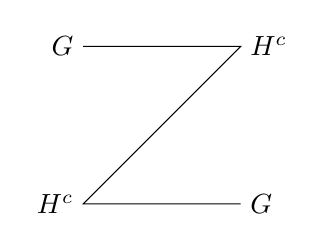
\begin{tikzpicture}
            \draw (0,0) node[left] {$G$} -- (2,0) node[right] {$H^c$} -- (0,-2) node[left] {$H^c$} -- (2,-2) node[right] {$G$};
        \end{tikzpicture}
    \end{figure}

    Now if $G \cong H$, it is easy to see $\Phi(G,H)$ is isomorphic to its complement.

    Conversely, if $\Phi(G,H) \cong \Phi(G,H)^c$, let $f$ be the witness of their isomorphism, and $d_1, d_2$ be the distance function on $\Phi(G,H)$ and $\Phi(G,H)^c$ respectively. Note that in $\Phi(G,H)$, $4\mathbb{N} \cup 4\mathbb{N}+3 = \{x \in \omega : \exists y \, d_1(x,y) = 3\}$. This is similar for $\Phi(G,H)^c$. So $f$ sends $4\mathbb{N} \cup 4\mathbb{N}+3$ to $4\mathbb{N}+1 \cup 4\mathbb{N}+2$. Also note that
    $$\{x \in \omega : \exists y \, (d_1(x,y) = 3) \land d_1(x,0) \leq 2\}$$
    is a copy of $G$,
    $$\{x \in \omega : \exists y \, (d_2(x,y) = 3) \land d_2(x,f(0)) \leq 2\}$$
    is a copy of $H$, and $f$ maps the former set to the latter set. So $G \cong H$.
\end{proof}

Using similar methods, Feng Li and Ruiwen Li also obtained the following:

\begin{theorem}
    The following sets are $\boldsymbol{\Sigma}^1_1$-complete:
    \begin{enumerate}
        \item The set of all countable directed graphs $G$ where $G \cong G^c$;
        \item The set of all countable tournaments $G$ where $G \cong G^c$.
    \end{enumerate}
\end{theorem}

A directed graph $G$ is a \emph{tournament} if for any distinct vertices $x, y \in G$, exactly one of $(x,y)$ and $(y,x)$ is an edge in $G$.

\subsection*{Some hyperfiniteness problems}
The following is the well-known Union Problem in the theory of hyperfinite equivalence relations.

\begin{problem}[The union problem]
    If $E$ is a countable Borel equivalence relation and $E = \cup_n F_n$, where $F_n$ is hyperfinite and $F_n \subseteq F_{n+1}$ for each $n \in \omega$, is it true that $E$ is hyperfinite?
\end{problem}

The following theorem was recently proved.

\begin{theorem}[Frisch--Shinko--Vidnyánszky \cite{FSV}]
    If there is a counterexample to the union problem, then the set of all hyperfinite equivalence relations is $\mathbf{\Sigma}_2^1$-complete.
\end{theorem}

Analogous to the above, we call a countable Borel equivalence relation \emph{hyperfinite-over-hyperfinite} (or shortly, \emph{hf/hf}) if there is a Borel partial order $\leq$ on $X$ such that
\begin{enumerate}[(i)]
    \item if $x \leq y$, then $x E y$,
    \item the order type of $\leq \upharpoonright_{[x]}$ is a suborder of $\mathbb{Z}^2$.
\end{enumerate}

\begin{problem}[The hf/hf problem]
    If $E$ is hf/hf, is it hyperfinite?
\end{problem}

There is an equivalent characterization for hyperfiniteness of hf/hf equivalence relation:
\begin{theorem}[Gao--Xiao \cite{GX}]
    If $E$ is hf/hf, then $E$ is hyperfinite iff $E$ admits a $\mathbb{Z}^2$ ordering which is self-compatible.
\end{theorem}

Inspired by the Frisch--Shinko--Vidnyánszky theorem, we ask:

\begin{problem}
    Suppose there is a counterexample to the hf/hf problem. Is the set of all hyperfinite equivalence relations $\mathbf{\Sigma}_2^1$-complete?
\end{problem}

\begin{bibentry}{9}
\begin{thebibliography}{9}
\bibitem{FSV} J. Frisch, F. Shinko, Z. Vidnyánszky, \textit{Hyper-hyperfiniteness and complexity}, preprint, 2024, arXiv: 2409.16445.
\bibitem{GX} S. Gao, M. Xiao, \textit{An order analysis of hyperfinite Borel equivalence relations}, Journal of Symbolic Logic, published online, DOI: 10.1017/jsl.2024.26.
\end{thebibliography}
\end{bibentry}
}


\section{Jing Yu}
%\abstractauthor{Jing Yu}
\abstractbody{
\begin{problem}[Weiss' question]
    Is the orbit equivalence relation of Borel action of countable amenable group hyperfinite?
\end{problem}

The orbit equivalence relations of actions of the following groups are proved to be hyperfinite:
\begin{quote}
    $\mathbb{Z}$ (Slaman--Steel),

    $\mathbb{Z}^n$ (Weiss),

    Groups of polynomial growth (Jackson--Kechris--Louveau),

    Abelian groups (Gao--Jackson),

    Locally nilpotent groups (Seward--Schneider),

    Polycyclic groups (Conley--Jackson--Marks--Seward--Tucker-Drob).
\end{quote}

Also the connected equivalence relations of the following graphs are proved to be hyperfinite:
\begin{quote}
    Graphs of polynomial growth (Bernshteyn--Yu),

    Graph of growth less than $\exp(r^c)$ for some small enough $0<c<1$ (Grebík--Marks--Rozhoň--Shinko).
\end{quote}

\begin{problem}
    How about graphs of uniform subexponential growth, i.e., of growth less than $\exp(r^c)$ for some $0<c<1$?
\end{problem}
}

\section{Riley Thornton}
%\abstractauthor{Riley Thornton}
\abstractbody{
Let $\text{Aut}([0,1],\lambda)$ denote the space of all automorphisms of the Lebesgue measure with the weak topology. Consider actions of $F_\infty$ on $[0,1]$ by automorphisms of Lebesgue measure.
Then the space of all such actions, $\text{Act}(F_\infty,([0,1],\lambda))$, is a closed subspace of $\text{Aut}([0,1],\lambda)^{F_\infty}$. 

For $x\in \text{Act}(F_\infty, ([0,1],\lambda))$, let $\mbox{Sch}(x)$ denote the Schreier graph of the action on $[0,1]$.

\begin{problem}
   Is the set
   $$\{x \in \text{Act}(F_\infty,([0,1],\lambda)) : \text{Sch}(x) \text{ has a measurable perfect matching}\}$$ 
   $\mathbf{\Sigma}_1^1$-complete?
\end{problem}

\begin{problem}[Halmos, 1956]
    What $T \in \text{Aut}([0,1],\lambda)$ has $S \in \text{Aut}([0,1],\lambda)$ with $T = S^2 = S \circ S$?

    Conjecture: $\{T \in \text{Aut}([0,1],\lambda) : \exists S \in \text{Aut}([0,1],\lambda) \, T = S^2\}$ is $\mathbf{\Sigma}_1^1$-complete.
\end{problem}
}

\section{Wei Dai}
%\abstractauthor{Wei Dai}
\abstractbody{
\begin{problem}
    If $\vec{G}$ is a Borel locally finite directed graph whose in-degrees are uniformly bounded and out-neighborhoods have polynomial growth, is the connected equivalence relation of $\vec{G}$ hyperfinite?
\end{problem}

\begin{problem}
    Let $\alpha$ be a free, probability measure preserving (p.m.p.) and ergodic action of $\mathbb{F}_2$ on measure space $(X,\mu)$.
    \begin{enumerate}[(i)]
        \item If $e \neq x \in \mathbb{F}_2$, is there a free, p.m.p action $\beta$ such that $E_\alpha = E_\beta$ and $x$ acts ergodically?
        \item (Miller--Tserunyan). Is there a free, p.m.p action $\beta$ such that every nontrivial element of $\mathbb{F}_2$ acts ergodically?
    \end{enumerate}
\end{problem}
}

\section{Jialiang He}
%\abstractauthor{Jialiang He}
\abstractbody{
A maximal eventually different family (MED) is a family $\mathlarger{\mathlarger{\varepsilon}} \subseteq \omega^\omega$ such that:
\begin{enumerate}[(i)]
    \item $\forall f \neq g \in \mathlarger{\mathlarger{\varepsilon}} \, |f \cap g| < \infty$ and
    \item $\forall f \in \omega^\omega \exists g \in \mathlarger{\mathlarger{\varepsilon}} \, |f \cap g| = \infty$.
\end{enumerate}

\begin{theorem}
    There exists a closed MED.
\end{theorem}

(Gao asked if there is a $\Pi^0_1$ MED.)

Let $I$ be an ideal on $\omega$. We can define $I$-MED analogous to the above definition. A family $\mathlarger{\mathlarger{\varepsilon}} \subseteq \omega^\omega$ is called an $I$-MED if:
\begin{enumerate}[(i)]
    \item For all $f \neq g \in \mathlarger{\mathlarger{\varepsilon}}$, $\{n : f(n) = g(n)\} \in I$ and
    \item $\forall h \in \omega^\omega \exists f \in \mathlarger{\mathlarger{\varepsilon}} \, \{n : f(n) = g(n)\} \in I^+$.
\end{enumerate}

\begin{theorem}
    If $I$ is an $F_\sigma$ ideal or $I = \text{Fin}^\alpha$, $\alpha < \omega_1$, then there exists a closed $I$-MED.
\end{theorem}

\begin{problem}
    For all Borel $I$, is there a closed $I$-MED?
\end{problem}

\begin{problem}
    For maximal ideal $I$, is there a closed $I$-MED?
\end{problem}

For these problems, it is enough to find a Borel $I$-MED.
\begin{theorem}
    For any ideal $I$, if there is a Borel $I$-MED, then there is a closed $I$-MED.
\end{theorem}
}
%\printaffiliations
\end{document}
